\section{Actividad No 01 – Manipulaci\'on de Datos} 

\begin{enumerate}[1.]
	\item El departamento de Recursos Humanos requiere crear sentencias SQL para insertar, actualizar y eliminar datos de empleados. Como prueba se utilizará la tabla Mis\_Empleados antes de remitir las sentencias al departamento de Recursos Humanos.

	\item Crear la tabla Mis\_Empleados utilizando la siguiente estructura.
	\begin{center}
	\includegraphics[width=5cm]{./Imagenes/imagen0102} 
	\end{center}
	\begin{center}
	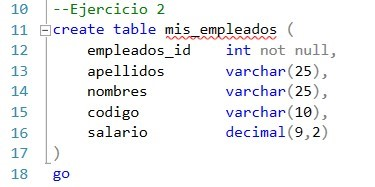
\includegraphics[width=8cm]{./Imagenes/img2} 
	\end{center}
	\item Generar una sentencia de inserción de datos que permita añadir los siguientes registros:
	\\
	\\ insert into mis\_empleados values (1, 'Vargas Canseco','Raúl', 'rvargas', 895),(2, 'Castro Feria',  'María','mcastro', 860);
	\\ go

	\begin{center}
	\includegraphics[width=8cm]{./Imagenes/imagen0103} 
	\end{center}
	\begin{center}
	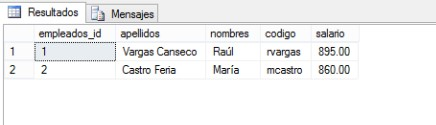
\includegraphics[width=12cm]{./Imagenes/img3} 
	\end{center}
	\item Generar un script que permita que mediante utilización de variables de sustitución, la inserción de información en la tabla Mis\_Empleados.
	\begin{center}
	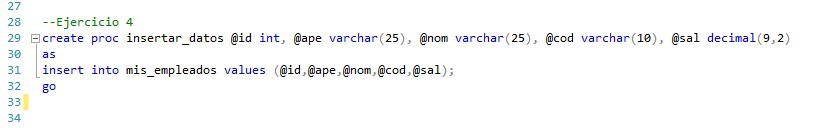
\includegraphics[width=18cm]{./Imagenes/img4} 
	\end{center}
	\item Utilizando el script anterior adicionar los siguientes registros.
	\begin{center}
	\includegraphics[width=5cm]{./Imagenes/imagen0105} 
	\end{center}
	\begin{center}
	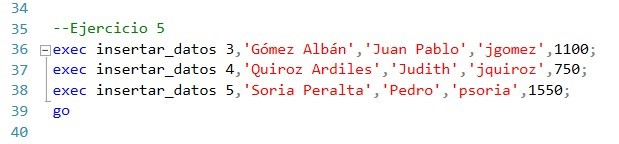
\includegraphics[width=18cm]{./Imagenes/img5} 
	\end{center}
	\item Revisar los cambios hechos a la tabla.
	\\
	\\ select * from mis\_empleados
	\\ go
	
	\begin{center}
	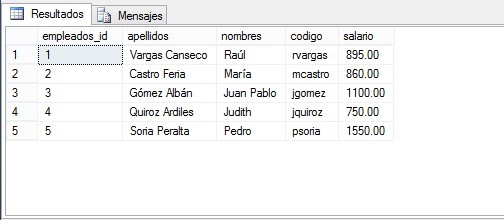
\includegraphics[width=10cm]{./Imagenes/img6} 
	\end{center}
	\item Cambiar el nombre del empleado No 3 a Benjamín.
	\\
	\\ update mis\_empleados set nombres='Benjamin' where empleados\_id=3;
	\\ go

	\begin{center}
	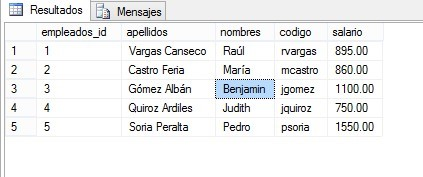
\includegraphics[width=10cm]{./Imagenes/img7} 
	\end{center}
	\item Elevar el salario a \$ 1,000 a todos los empleados que tengan un salario menor a esa cantidad.
	\\
	\\ update mis\_empleados set salario=1000 where salario<1000;
	\\ go

	\begin{center}
	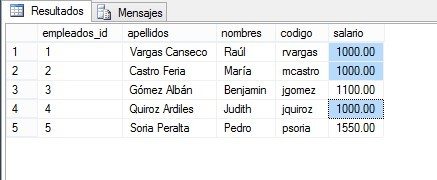
\includegraphics[width=10cm]{./Imagenes/img8} 
	\end{center}
	\item Eliminar el registro del empleado María Castro
	\\
	\\ delete from mis\_empleados where codigo='mcastro';
	\\ go

	\begin{center}
	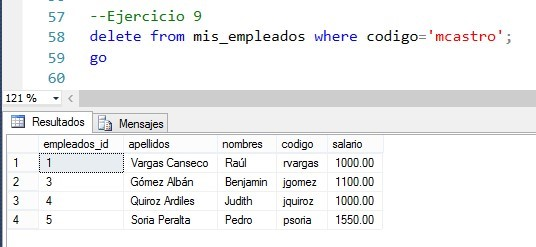
\includegraphics[width=10cm]{./Imagenes/img9} 
	\end{center}
	\item Revisar los cambios hechos a la tabla.
	\\
	\\ select [Begin Time],[RowLog Contents 1],[Transaction Name],Operation 
	\\from sys.fn\_dblog(NULL,NULL) 
	\\where AllocUnitName='dbo.mis\_empleados' and Operation IN ('LOP\_DELETE\_ROWS')
	\\ go

	\begin{center}
	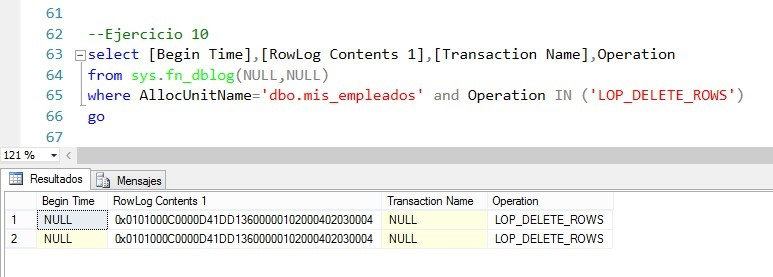
\includegraphics[width=10cm]{./Imagenes/img10} 
	\end{center}
	\item Confirmar los cambios a la tabla.
	\\
	\\ select * from mis\_empleados
	\\ go

	\begin{center}
	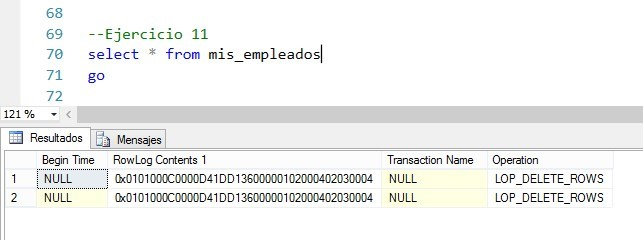
\includegraphics[width=10cm]{./Imagenes/img11} 
	\end{center}
	\item Adicionar el siguiente registro a la tabla
           \\
	\\exec insertar\_datos 6,'Hurtado Gamboa','Ernesto','ehurtado',1400
	\\ go

	\begin{center}
	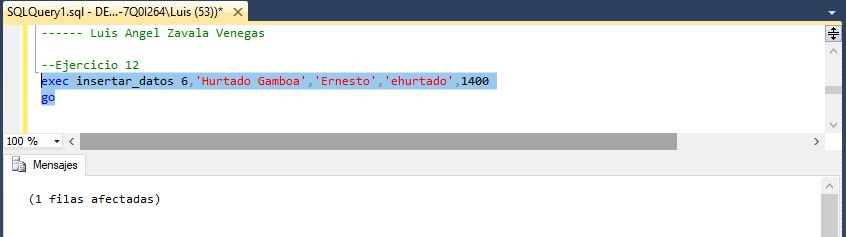
\includegraphics[width=10cm]{./Imagenes/1ejer12} 
	\end{center}
	\item Revisar la adición realizada
          \\
	\\select * from mis\_empleados
	\\ go

	\begin{center}
	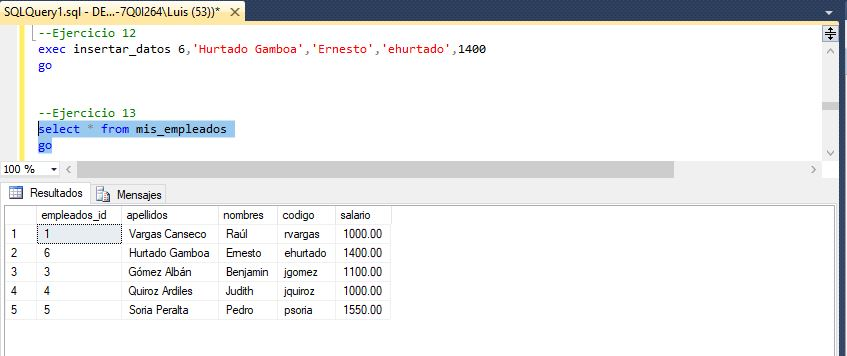
\includegraphics[width=10cm]{./Imagenes/1ejer13} 
	\end{center}

	\item Crear un punto de restauración intermedio para esta transacción
          \\
	\\begin tran;
           \\save tran p1;
	\begin{center}
	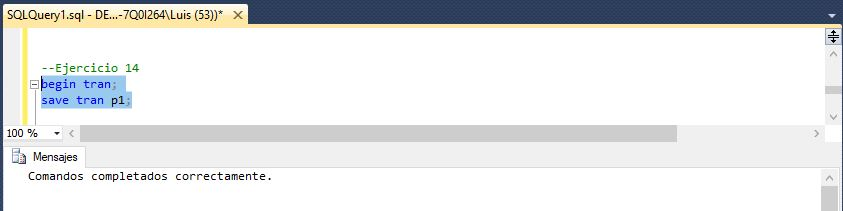
\includegraphics[width=10cm]{./Imagenes/1ejer14} 
	\end{center} 

	\item Borrar los registros de la tabla MIS\_EMPLEADOS.
          \\
	\\delete from mis\_empleados;
	\begin{center}
	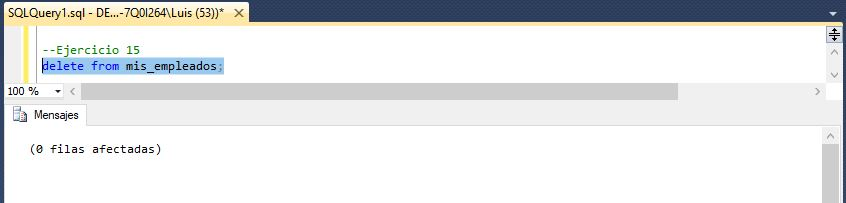
\includegraphics[width=10cm]{./Imagenes/1ejer15} 
	\end{center}

	\item Revisar los cambios realizados.
	\item Descartar los cambios hechos a la tabla sin descartar la última adición hecha.
	\item Revisar nuevamente los registros de la tabla MIS\_EMPLEADOS.
	\item Confirmar todos los cambios hechos a la tabla MIS\_EMPLEADOS.
	\item Modificar el script del punto 4.4. a fin de que se genere automáticamente el CODIGO del empleado que lo conforman la primera letra de su nombre y la primera palabra de su apellido.
	\item Adicionar el siguiente registro a la tabla a fin de corroborar el funcionamiento del script anterior
	\item Revisar los cambios realizados. Y finalmente confirmar todos los cambios hechos a la tabla MIS\_EMPLEADOS.

\end{enumerate} 
